\documentclass{article}
\usepackage{array}
\usepackage{graphicx}
\usepackage{amsmath, amsthm, thmtools, mathdots, mathtools, amssymb}
\usepackage[pdfusetitle]{hyperref}
\usepackage[all]{hypcap} % Links hyperref to object top and not caption
\usepackage[nameinlink]{cleveref}   
\usepackage{makecell, multirow, booktabs}
\usepackage{caption, subcaption}
\usepackage{float}
\usepackage[bottom]{footmisc}
\usepackage[inline]{enumitem}
\usepackage{appendix}
\usepackage{biblatex}
\addbibresource{references.bib}
\hypersetup{ colorlinks, citecolor=black, filecolor=black, linkcolor=black, urlcolor=black, linktoc=all }
\newcommand*\rot{\rotatebox{90}}

\let\endtitlepage\relax

\newtheorem{theorem}{Theorem}
\newtheorem{definition}{Definition}
\newtheorem{lem}{Claim}


\begin{document}
    \begin{titlepage}
        \begin{center}
            {\LARGE Multiple Couriers Problem}
            \vspace*{1em}
            
            Valerio Costa, Luca Domeniconi, Claudia Maiolino, Tian Cheng Xia

            \centerline{\{valerio.costa, luca.domeniconi5, claudia.maiolino, tiancheng.xia\}@studio.unibo.it}
        \end{center}
    \end{titlepage}

    \thispagestyle{plain}

    \section{Introduction} \label{sec:intro}
    The problem of this project is known in the literature as the capacitated vehicle routing problem and can be easily proven to be NP-hard. We tackle this problem by virtually splitting it into two sub-problems: first we look for an assignment of the items to the couriers and then search for the routes of each of them (i.e., by solving multiple traveling salesman problems). To solve the latter, we follow the approach presented in \cite{vrp} where the route of a courier is modelled through the variables $P_d \in [1, n+1]$ with $d \in [1, n+1]$ defined as follows:
    \begin{equation}
        \label{eq:path_def}
        P_{d_1} = \begin{cases}
            d_2 & \text{iff the location $d_2 \neq d_1$ is visited immediately after $d_1$}\\
            d_1 & \text{iff $d_1$ is not part of the route of the courier}
        \end{cases}
    \end{equation} 
    With proper assignment and subtour elimination constraints, $P_d$ allows to define a Hamiltonian cycle that passes through the items that the courier delivers and the solution can be extracted by traversing the cycle starting from the depot $n+1$.

    The lower-bound of the objective function is common to all models and is defined as the maximum path cost that involves a single package:
    \begin{equation}
        \max_{p \in [1, n]} \left\{ D_{n+1, p} + D_{p, n+1} \right\}
    \end{equation}

    As upper-bound, also common to all models, we observed that it does not provide any improvement to the results. Nevertheless, we defined it as:
    \begin{equation}
        \sum_{d_1 \in [1, n+1]} \max_{d_2 \in [1, n+1]} D_{d_1, d_2}
    \end{equation}

    Symmetry breaking constraints are also common to all models. By considering couriers with the same capacity, the following constraints can be used to avoid symmetries:
    \begin{itemize}
        \item By imposing an ordering on the amount of assigned packages:
            \begin{equation}
                \label{eq:cp_symm_amount}
                \forall c_1, c_2 \in [1, m]: (c_1 < c_2 \land l_{c_1} = l_{c_2}) \Rightarrow Q_{c_1} \leq Q_{c_2}
            \end{equation}
            where $Q_c$ is the amount of packages delivered by the courier $c$.
        \item By imposing an ordering on the indexes of the assigned packages:
            \begin{equation}
                \label{eq:cp_symm_packs}
                \forall c_1, c_2 \in [1, m]: (c_1 < c_2 \land l_{c_1} = l_{c_2}) \Rightarrow A_{c_1} <_\texttt{lex} A_{c_2}
            \end{equation}
            where $A_c$ is an ordered vector containing the packages delivered by the courier $c$.
    \end{itemize}

    As the triangle inequality holds, we also identified an implied constraint that consists of imposing that each courier delivers at least a package (a short proof is provided in \Cref{sec:impl_proof}):
    \begin{equation}
        \label{eq:impl_constr}
        \forall c \in [1, m]: Q_c \geq 1  
    \end{equation}
    where $Q_c$ is the amount of packages delivered by the courier $c$.
    This obviously is applicable only if each courier is able to carry at least an item.

    All experiments were done using the same random seed and were run as workflows on GitHub Actions which provides two cores at 2.45 GHz and 7 GB of memory. To guarantee a safe margin for the Docker container to run, the actual usable memory was capped to 5 GB.

    The work has been completed in approximately one month and has been roughly split in the following way: Xia did the CP part, Costa worked on SAT, Domeniconi did the SMT models, and Maiolino completed the MIP part. The main difficulties we encountered are the following: 
    \begin{enumerate*}[label=(\roman*)]
        \item lack of proper documentation for many tools we used,
        \item difficulties to find a more efficient way to solve bigger instances,
        \item the need of time to run the experiments on all instances.
    \end{enumerate*}


    \section{CP model}


\subsection{Decision variables}

The CP model relies on the following decision variables:
\begin{itemize}
    \item For each package $p$, $A_p \in [1, m]$ (\texttt{assignments[p]} in MiniZinc) indicates which courier delivers it. More specifically, $A_p = c$ iff the package $p$ is delivered by the courier $c$.
    
    \item For each courier $c$, $P_{c, d}$ (\texttt{path[c, d]} in MiniZinc) is defined following \Cref{eq:path_def}.
\end{itemize}



\subsection{Objective function}
Once the route of each courier has been found, the objective function is computed as follows:
\begin{equation}
    \max_{c \in [1, m]} \sum_{\substack{d \in [1, n+1]:\\P_{c, d} \neq d}} D_{d, P_{c, d}}
\end{equation}


\subsection{Constraints}

To respect the capacity limit of each courier, the following constraint can be defined:
\begin{equation}
    \forall c \in [1, m]: \sum_{p \in [1, n]: A_p = c} s_p \leq l_c 
\end{equation}
In MiniZinc, the global constraint \texttt{bin\_packing\_capa} also models this. In our experiments, we did not notice significant differences between the two formulations and decided to use the latter following the best practice of preferring global constraints.

To model the route, the following constraints have to be imposed:
\begin{equation}
    \label{eq:cp_constr_route_depot}
    \forall c \in [1, m]: 
    \begin{cases}
        P_{c, n+1} = n+1    & \text{if $\nexists p \in [1, n]: A_p = c$} \\ 
        P_{c, n+1} \neq n+1 & \text{if $\exists p \in [1, n]: A_p = c$} 
    \end{cases}
\end{equation}

\begin{equation}
    \label{eq:cp_constr_route_packs}
    \forall c \in [1, m],
    \forall p \in [1, n]: 
    \begin{cases}
        P_{c, p} = p    & \text{if $A_p \neq c$} \\
        P_{c, p} \neq p & \text{if $A_p = c$} 
    \end{cases}
\end{equation}

The constraint defined in \Cref{eq:cp_constr_route_depot} imposes that, for each courier, the depot has a successor only if that courier delivers at least a package. On the same note, \Cref{eq:cp_constr_route_packs} imposes that only the packages delivered by a specific courier have a successor in the route.
Moreover, it is necessary to impose that the route defined by $P_c$ is a Hamiltonian cycle that passes through the relevant destinations. In MiniZinc, this can be easily modelled by using the global constraint \texttt{subcircuit}.


\subsubsection{Symmetry breaking constraints}

For CP, we experimented with both symmetry breaking constraints defined in \Cref{eq:cp_symm_amount,eq:cp_symm_packs}. Moreover, we experimented with a stronger version of these constraints that is applied between two couriers whose actual loads are interchangeable. This is defined by the following condition:
\begin{equation}
    \label{eq:cp_symm_strong}
    \max\left\{ L_{c_1}, L_{c_2} \right\} \leq \min\left\{ l_{c_1}, l_{c_2} \right\}
\end{equation}
where $L_c$ is the actual load carried by the courier $c$.



\subsection{Validation}

\subsubsection{Experimental design}

We experimented variations of our models using as solvers Gecode, Chuffed, and OR-Tools. The search order for all models assigns the packages (\texttt{assignments}) first and then searches for the route (\texttt{path}) of each courier in decreasing order of capacity. Regarding search, we experimented several combinations of variable selection and assignment strategies on a subset of instances and only used the best ones to obtain the final complete results.


\subsubsection{Experimental results}

From some preliminary experiments, we observed that first fail and largest domain with weighted degree (\texttt{dom\_w\_deg}) are the best performing search strategies. Therefore, we performed the full experiments using as search strategy \texttt{dom\_w\_deg} for \texttt{assignments} and \texttt{first\_fail} for \texttt{path}, respectively. Moreover, between the two symmetry breaking constraints, we observed that the lexicographic ordering defined in \Cref{eq:cp_symm_packs} has better performances and therefore present only those results. The objective values found by the most significant models are reported in \Cref{tab:cp_results}.

\begin{table}[ht]
    \caption{Selected subset of CP results. Results in \textbf{bold} are solved to optimality. Instances that are all solved to optimality have been omitted.}
    \label{tab:cp_results}
    \centerline{
        \begin{tabular}{c|cccccccccccc}
            \toprule
            & \multicolumn{6}{c}{Gecode} & \multicolumn{3}{c}{Chuffed} & \multicolumn{3}{c}{OR-Tools} \\
            \\[-3ex] % Remove vertical line gap
            \cmidrule(lr){2-7} \cmidrule(lr){8-10} \cmidrule(lr){11-13}
            Id & \rot{plain}    & \rot{luby}    & \rot{lns80}   & \rot{lns95}   & \rot{\makecell[l]{lns95\\[-0.3em]\small+ SB \eqref{eq:cp_symm_packs}}} & \rot{\makecell[l]{lns95\\[-0.3em]\small+ SB \eqref{eq:cp_symm_packs}\eqref{eq:cp_symm_strong}}} & \rot{plain} & \rot{luby} & \rot{SB \eqref{eq:cp_symm_packs}} & \rot{plain} & \rot{\makecell[l]{plain\\[-0.3em]\small+ FS}} & \rot{\makecell[l]{SB \eqref{eq:cp_symm_packs}\\[-0.3em]\small+ FS}} \\ 
            \midrule
            7  & 201            & \textbf{167}  & \textbf{167}  & \textbf{167}  & \textbf{167}  & \textbf{167}  & \textbf{167}  & \textbf{167}  & \textbf{167}  & 408           & \textbf{167}  & \textbf{167}  \\ 
            9  & \textbf{436}   & \textbf{436}  & \textbf{436}  & \textbf{436}  & \textbf{436}  & \textbf{436}  & \textbf{436}  & \textbf{436}  & \textbf{436}  & 617           & \textbf{436}  & \textbf{436}  \\ 
            11 & 594            & 597           & 528           & 490           & 503           & --            & 963           & --            & 756           & 1669          & 1189          & 1081          \\ 
            12 & 449            & 428           & 375           & \textbf{346}  & 348           & --            & 833           & 1061          & 785           & 1605          & 706           & 899           \\ 
            13 & 648            & 704           & 656           & 616           & 610           & 624           & 1126          & 914           & 1126          & 1734          & 584           & 746           \\ 
            14 & 725            & 972           & 794           & 715           & 792           & --            & 1449          & --            & 1089          & --            & --            & --            \\ 
            15 & 659            & 901           & 765           & 738           & 803           & --            & 1292          & --            & --            & --            & --            & --            \\ 
            16 & 451            & 294           & \textbf{286}  & \textbf{286}  & \textbf{286}  & --            & 487           & 636           & 694           & 998           & 467           & 363           \\ 
            17 & 1324           & 1468          & 1119          & 1076          & 1155          & --            & --            & --            & --            & --            & --            & --            \\ 
            18 & 691            & 806           & 675           & 662           & 620           & --            & 1321          & --            & 1779          & --            & --            & --            \\ 
            19 & 554            & 412           & 336           & \textbf{334}  & \textbf{334}  & --            & 795           & 1079          & 765           & 1521          & 623           & 577           \\ 
            20 & 1139           & 1369          & 1104          & 1068          & 1075          & --            & --            & --            & --            & --            & --            & --            \\ 
            21 & 779            & 687           & 600           & 516           & 529           & --            & 2104          & 2140          & 993           & 2115          & 1226          & --            \\ 
            \bottomrule
        \end{tabular}
    }
\end{table}

For Gecode, we experimented different search approaches by testing restart methods, large neighborhood search (LNS), and varying symmetry breaking constraints. We observed that, compared to a depth-first approach, by simply restarting search following the Luby sequence there is a mixed impact on the results with both positive and negative effects. Instead, by also using LNS, results tend to improve globally and we observed that a higher retain probability, with a peak at around $95\%$, works better. Regarding symmetry breaking constraints, we observed that they tend to worsen the final objective value in the majority of the cases, most reasonably due to the fact that the overhead to impose them is higher than the speed-up in search. For a visual comparison, we show in \Cref{fig:cp_obj_plots} the evolution of the objective value during search. It can be seen that without restart the objective stops improving in the early stages of search as it most likely gets ``stuck" in a branch of the search tree. By introducing some non-determinism, the objective reaches lower values, with LNS being the fastest and best performing.

\begin{figure}[H]
    \centering
    \begin{subfigure}{0.49\linewidth}
        \centering
        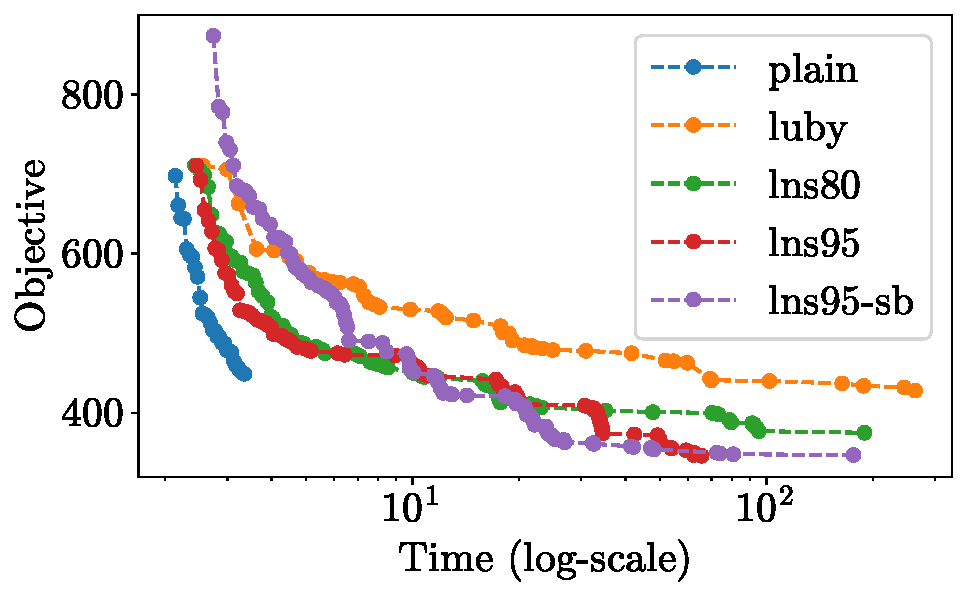
\includegraphics[width=\linewidth]{img/cp/obj-plot_inst12.pdf}
        \caption{Instance 12}
    \end{subfigure}
    \hfill
    \begin{subfigure}{0.49\linewidth}
        \centering
        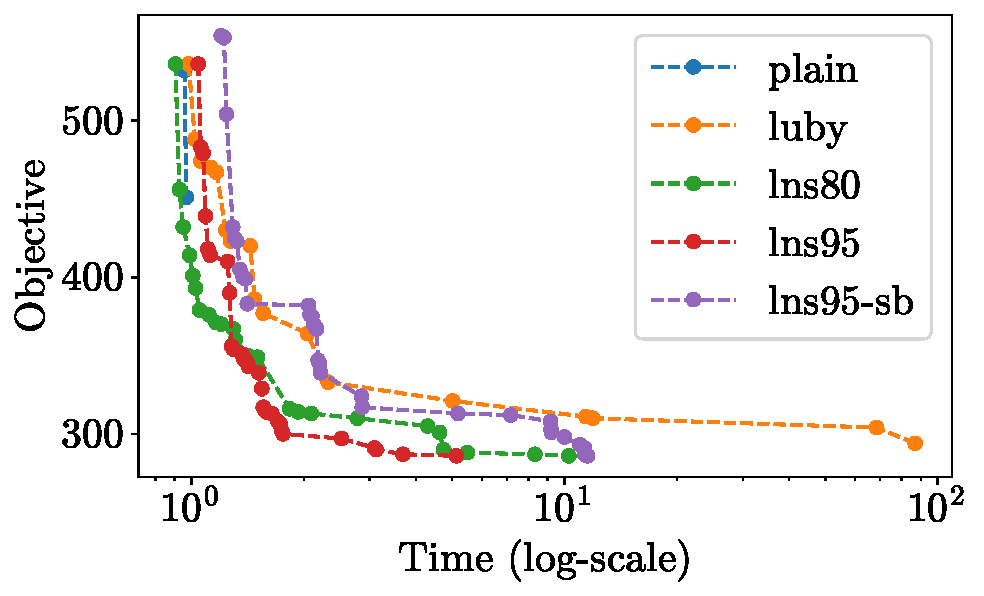
\includegraphics[width=\linewidth]{img/cp/obj-plot_inst16.pdf}
        \caption{Instance 16}
    \end{subfigure}
    \caption{Intermediate solutions using Gecode}
    \label{fig:cp_obj_plots}
\end{figure}

For Chuffed, we only experimented with restarts and symmetry breaking constraints as LNS is not available through MiniZinc. Moreover, as indicated in the documentation\footnote{\url{https://docs.minizinc.dev/en/stable/solvers.html}}, we tried enabling free search mode but only obtained worse results. Compared to Gecode, results on bigger instances are generally all worse, while smaller instances tend to be solved faster by Chuffed. As in Gecode, restarts, which we only experimented with random variable selection as it is the only non-deterministic search strategy available, and symmetry breaking constraints both yield mixed effects on the final result.

Finally, for OR-Tools, we conducted fewer experiments as it supports fewer MiniZinc annotations. In this case, we observed that enabling free search mode allows obtaining better results and, similarly to Gecode and Chuffed, symmetry breaking constraints have mixed results. As a side note, we must also observe that, as suggested in the documentation, these results are worse as OR-Tools performs better with multi-threading. 


    \section{SAT model}

The resolution of the problem is approached following two models.

\begin{itemize}
    \item \textbf{Unified model}:
    based on the definition of two decision variables \texttt{assignments} and \texttt{paths}.
    \item \textbf{Matrix model}:
    based on the definition of one decision variable $X$.
\end{itemize}

Some modifications were applied to those model in order to visualize eventual differences in terms of performances.

The discussion is going to be much more focused on the Unified model just to mantain a logical thread within the explication of models used for other solvers.

\subsection{Unified Model}

\paragraph*{General Definition}
The Unified model aims to find the correct assignment to both decision variables, in such a way that it satisfy all constraints.\\
The idea behind this kind of model is based on the separation of the two task just specified in one.

\paragraph*{Original Workflow}
The original workflow follows the next steps:
\begin{enumerate}
    \item find satisfying values for the \texttt{assignments} variable, else end the algorithm
    \item find satisfying values for the \texttt{paths} variable, else proceed to step $4$
    \item repeat step $2$ to find a new optimized solution,
    \item repeat step $1$ just to find another assignment
\end{enumerate}

\paragraph*{New Workflow}
The new algorithm simply tries to optimize the assignment to both variable.

\paragraph*{Pro}
The model was designed to improve certain intrinsic problems of the definition of a problem through SAT:
\begin{itemize}
    \item \textbf{Specificity of constraints}: constraining much more the assignments of the two variable guarantes to mantain lower width of exploration of the resolution tree.
\end{itemize} 

\paragraph*{Contro}
The model falls into a few issues such:

\begin{itemize}
    \item \textbf{Dimension}: being based on two decision variables, the dimension of the problem scale exponentially with them. \footnote{The scaling dimension of the problem implies higher needs of time to build the model.}
\end{itemize}

\subsubsection{Decision variables}

\begin{itemize}
    \item \texttt{assignments}: $n \times m$ boolean matrix
    \begin{equation}
        \label{eq:assignments}
        \texttt{assignments[$p$, $c$] = 1 }
        % \quad
        % \texttt{if courier $c$ delivers pack $p$}
    \end{equation}
    \begin{center}
        \texttt{if courier $c$ delivers pack $p$}
    \end{center}

    \item \texttt{paths}: $m \times (n+1) \times (n+1)$ boolean matrix
    \begin{equation}
        \label{eq:paths}
        \texttt{paths[$c$, $loc_1$, $loc_2$] = 1 }
    \end{equation}
    \begin{center}
        \texttt{if courier $c$ moves from location $loc_1$ to $loc_2$}
    \end{center}

    \item \texttt{u}: $m \times n \times n$ boolean matrix\footnote{The definition of the \texttt{u} variable is useful for the MTZ formulation.}
    \begin{equation}
        \label{eq:u}
        \texttt{u[$c$, $p_1$, $p_2$] = 1 }
    \end{equation}
    \begin{center}
        \texttt{if in the courier $c$ path the node $p_1$ is associated to value $p_2$}
    \end{center}
    
\end{itemize}

\subsubsection{Objective function}

The model aims to minimize the maximum distance travelled by any courier.
The objective function can estimated as the maximum between the total distances of each courier:

\begin{equation}
    \label{eq:obj_fun}
    \max_{c \in \{ 1, \dots, m \}}
    \sum_{loc_1=1}^{n+1} \sum_{loc_2=1}^{n+1} \texttt{D[$loc_1$, $loc_2$]}*
    \texttt{paths[$c$, $loc_1$, $loc_2$]}
\end{equation}

A lower bound is set to costrain the objective during the resolution phase.
\begin{equation}
    \label{eq:lower_bound}
    \max_{p \in \{ 1, \dots, n \}}
    \texttt{D[$n+1$, $p$] + D[$p$, $n+1$]}
\end{equation}
Its value is hypotesized to be the maximum between the minimum distance paths that a courier can travel. And this can be computed as the distance needed for a courier to reach a certain pack and return to the depot.



\subsubsection{Constraints}

\paragraph*{Assignment related constraints}

\begin{itemize}
    \item Capacity constraint:
    \begin{itemize}
        \item Sum of sizes of packs delivered by a singular courier must be under its load limit
        \begin{equation}
            \label{eq:capacity1}
            \forall c \in \{1 \ldots m\}:
            \quad
            \sum_{p=1}^{n} \texttt{assignments[$p$, $c$] * sizes[$p$]} \leq \texttt{loads[$c$]}
        \end{equation}
        \item Each pack must be delivered only by a courier
        \begin{equation}
            \label{eq:capacity2}
            \forall p \in \{1, \ldots, n\}: \exists! c \in \{1, \ldots, m\} \quad \texttt{s.t.} \quad \texttt{assignments[$p$, $c$]} = \texttt{1}
        \end{equation}
    \end{itemize}
\end{itemize}

\paragraph*{Path related constraints}

\begin{itemize}
    \item General path constraints
    \begin{itemize}
        \item If courier delivers at least one package, there must exist a destination from DEPOT\footnote{DEPOT is the original position, hypotesized as \texttt{n+1}.} with true value, else it can stay in DEPOT
        \begin{equation}
            \label{eq:gen_path_constr1}
            \forall c \in \{1 \ldots m\}:
            \forall p \in \{1 \ldots n\}:
            \left\{
                \begin{array}{lr}
                    \texttt{NOT(paths[$c$, DEPOT, DEPOT])} & \texttt{iff } \sum_{p=1}^{n} \texttt{assignments[$p$, $c$]} \geq \texttt{1}\\
                    \texttt{paths[$c$, DEPOT, DEPOT]} & \texttt{iff } \sum_{p=1}^{n} \texttt{assignments[$p$, $c$]} = \texttt{0} % or otherwise
                \end{array}
            \right\}
        \end{equation}

        \item If courier delivers pack p, its destination must be different from p 
        \begin{equation}
            \label{eq:gen_path_constr2}
            \forall c \in \{1 \ldots m\}:
            \forall p \in \{1 \ldots n\}:
            \left\{
                \begin{array}{lr}
                    \texttt{NOT(paths[$c$, $p$, $p$])} & \texttt{iff } \texttt{assignments[$p$, $c$]}\\
                    \texttt{paths[$c$, $p$, $p$]} & \texttt{iff } \texttt{NOT(assignments[$p$, $c$])} % or otherwise
                \end{array}
            \right\}
        \end{equation}

        \item Each pack must be delivered by a single courier only once
        \begin{equation}
            \label{eq:gen_path_constr3}
            \forall c \in \{1 \ldots m\}:
            \forall loc_1 \in \{1 \ldots n+1\}:
            \quad
            \sum_{loc_2=1}^{n+1} \texttt{paths[$c$, $loc_1$, $loc_2$]} = \texttt{1}
        \end{equation}
    \end{itemize}
    \item Subcircuit constraints
    \begin{itemize}
        \item Only a single courier must deliver pack in location $loc_2$ from $loc_1$
        \begin{equation}
            \label{eq:subtour_constr1}
            \forall c \in \{1 \ldots m\}:
            \forall loc_2 \in \{1 \ldots n+1\}:
            \quad
            \sum_{loc_1=1}^{n+1} \texttt{paths[$c$, $loc_1$, $loc_2$]} = \texttt{1}
        \end{equation}
        \item Subtour elimination
        \begin{itemize}
            \item $u$ relative to first pack $p$ of courier $c$ path must have value = 1
            \begin{equation}
                \label{eq:subtour_constr2}
                \forall c \in \{1 \ldots m\}:
                \forall p \in \{1 \ldots n\}:
                \quad
                \texttt{iff}
                \quad
                \texttt{paths[$c$, DEPOT, $p$]}
                \quad
                \texttt{then}
                \quad
                \texttt{u[$c$, $p$, $1$]}
            \end{equation}
            \item $u_j \geq u_i + 1$
            \begin{equation}
                \label{eq:subtour_constr3}
                \forall c \in \{1, \dots, m\}: \ \forall i, j, k \in \{1, \dots, n\}: \quad
                \texttt{paths}[c, i, j] \land \texttt{u}[c, i, k] \Longrightarrow
                \sum_{l=k+1}^{n} \texttt{u}[c, j, l] = 1
            \end{equation}
            
            \item Exatcly one true value for each \texttt{u[$c, p, :$]} vector
            \begin{equation}
                \label{eq:subtour_constr4}
                \forall c \in 1 \ldots m:
                \forall p_1 \in 1 \ldots n:
                \quad
                \sum_{p_2=1}^{n} \texttt{u[$c$, $p_1$, $p_2$]} = \texttt{1}
            \end{equation}

            \item MTZ formulation constraint:
            \begin{center}
                $u_i - u_j + 1 \leq (n - 1)$ * $(1 - paths[c, i, j] )$
            \end{center}
            \begin{equation}
                \label{eq:subtour_constr5}
                \forall c \in \{1, \dots, m\}, \ \forall i, j, k_1, k_2 \in \{1, \dots, n\}: 
            \end{equation}
            \begin{center}\[
                \quad
                \texttt{u}[c, i, k_1] \land \texttt{u}[c, j, k_2] \Longrightarrow
                (k_1 - k_2 + 1) \leq (n-1) \cdot (1 - \texttt{paths}[c, i, j])
                \]
            \end{center}
        \end{itemize}
    \end{itemize}
\end{itemize}

\paragraph*{Symmetry breaking constraint}

A possible way to reduce tree exploration is to introduce symmetry breaking constraints.
One of them in this case can consist in constraining the order of assignments of packs between couriers with the same amount of load capacity.

But the experimentation didn't lead to major improvements.

\subsection{Validation}

\subsubsection*{Experimental design}

Some modifications were applied to the basic model in order to visualize eventuale differences in performances.
The original Unified Model was modified in three different versions:
\begin{itemize}
    \item Unified Model with Symmetry Breaking Constraint
    \item Unified Model with Cumulative Constraint Application
    \item Unified Model with Heule Encoding approach for \texttt{at\_most\_one()}
\end{itemize}
\subsubsection*{Experimental results}

As we can notice from the following table the performances were not very much different from the basic model. Only in the first 10 instances it has been possible to rach at least a suboptimal solution, while for the remaining ones the construction of the model required too much time causing the exceeding of the timeout limit.
\begin{table}[h]
    \centering
    \begin{tabular}{cccccc}
            \toprule
            Id & un-model & un-symm-model & un-cum-constr-model & un-heule-enc-model & matrix-model \\ 
            \midrule
            1 & \textbf{14} &       \textbf{14} &   \textbf{14} &   \textbf{14} &   \textbf{14} \\ 
            2 & \textbf{226} &      \textbf{226} &  \textbf{226} &  \textbf{226} &  \textbf{226} \\ 
            3 & \textbf{12} &       \textbf{12} &   \textbf{12} &   \textbf{12} &   \textbf{12} \\ 
            4 & \textbf{220} &      \textbf{220} &  \textbf{220} &  \textbf{220} &  \textbf{220} \\ 
            5 & \textbf{206} &      \textbf{206} &  \textbf{206} &  \textbf{206} &  \textbf{206} \\ 
            6 & \textbf{322} &      \textbf{322} &  \textbf{322} &  \textbf{322} &  \textbf{322} \\ 
            7 & 232 &       238 &   222 &   296 &   292 \\ 
            8 & \textbf{186} &      \textbf{186} &  \textbf{186} &  \textbf{186} &  \textbf{186} \\ 
            9 & \textbf{436} &      \textbf{436} &  \textbf{436} &  \textbf{436} &  \textbf{436} \\ 
            10 & \textbf{244} &     \textbf{244} &  \textbf{244} &  \textbf{244} &  \textbf{244} \\ 
            11 & -- &       -- &    -- &    -- &    -- \\ 
            12 & -- &       -- &    -- &    -- &    -- \\ 
            13 & -- &       -- &    -- &    -- &    -- \\ 
            14 & -- &       -- &    -- &    -- &    -- \\ 
            15 & -- &       -- &    -- &    -- &    -- \\ 
            16 & -- &       -- &    -- &    -- &    -- \\ 
            17 & -- &       -- &    -- &    -- &    -- \\ 
            18 & -- &       -- &    -- &    -- &    -- \\ 
            19 & -- &       -- &    -- &    -- &    -- \\ 
            20 & -- &       -- &    -- &    -- &    -- \\ 
            21 & -- &       -- &    -- &    -- &    -- \\ 
            \bottomrule
    \end{tabular}
    \caption{Objective value through instances}
\end{table}


\begin{figure}[H]
    \centering
    \begin{subfigure}{0.49\linewidth}
        \centering
        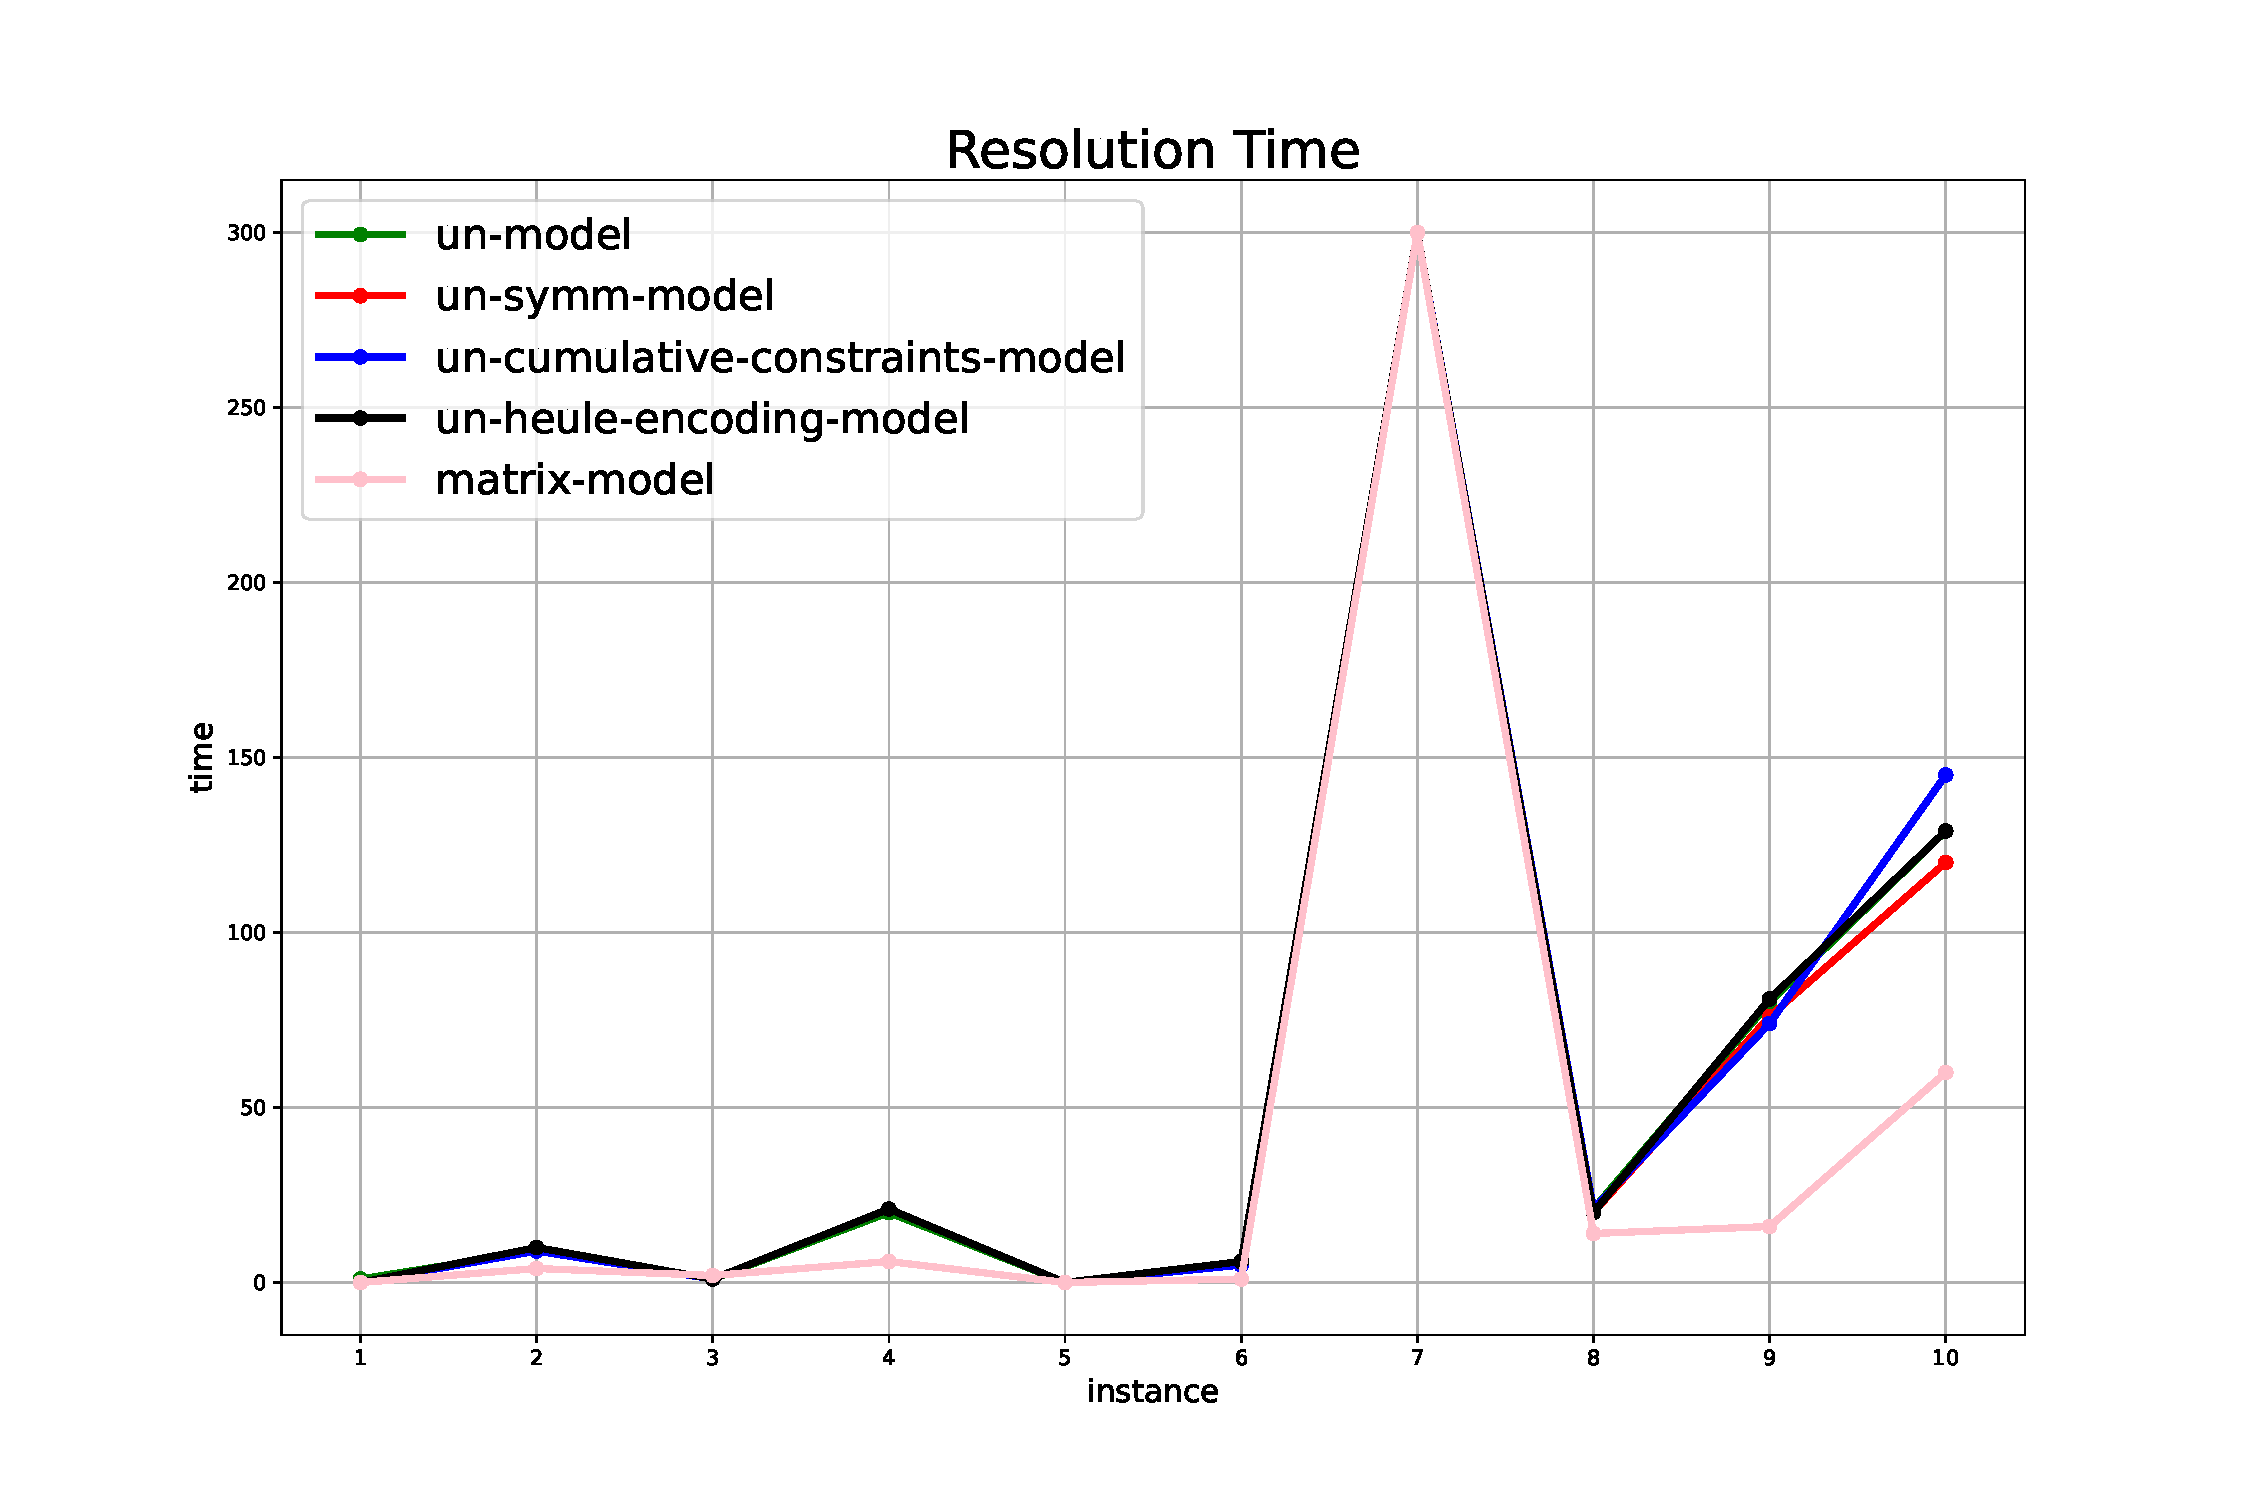
\includegraphics[width=\linewidth]{sat_images/time.pdf}
        \caption{Resolution time for each instance}
    \end{subfigure}
    \hfill
    \centering
    \begin{subfigure}{0.49\linewidth}
        \centering
        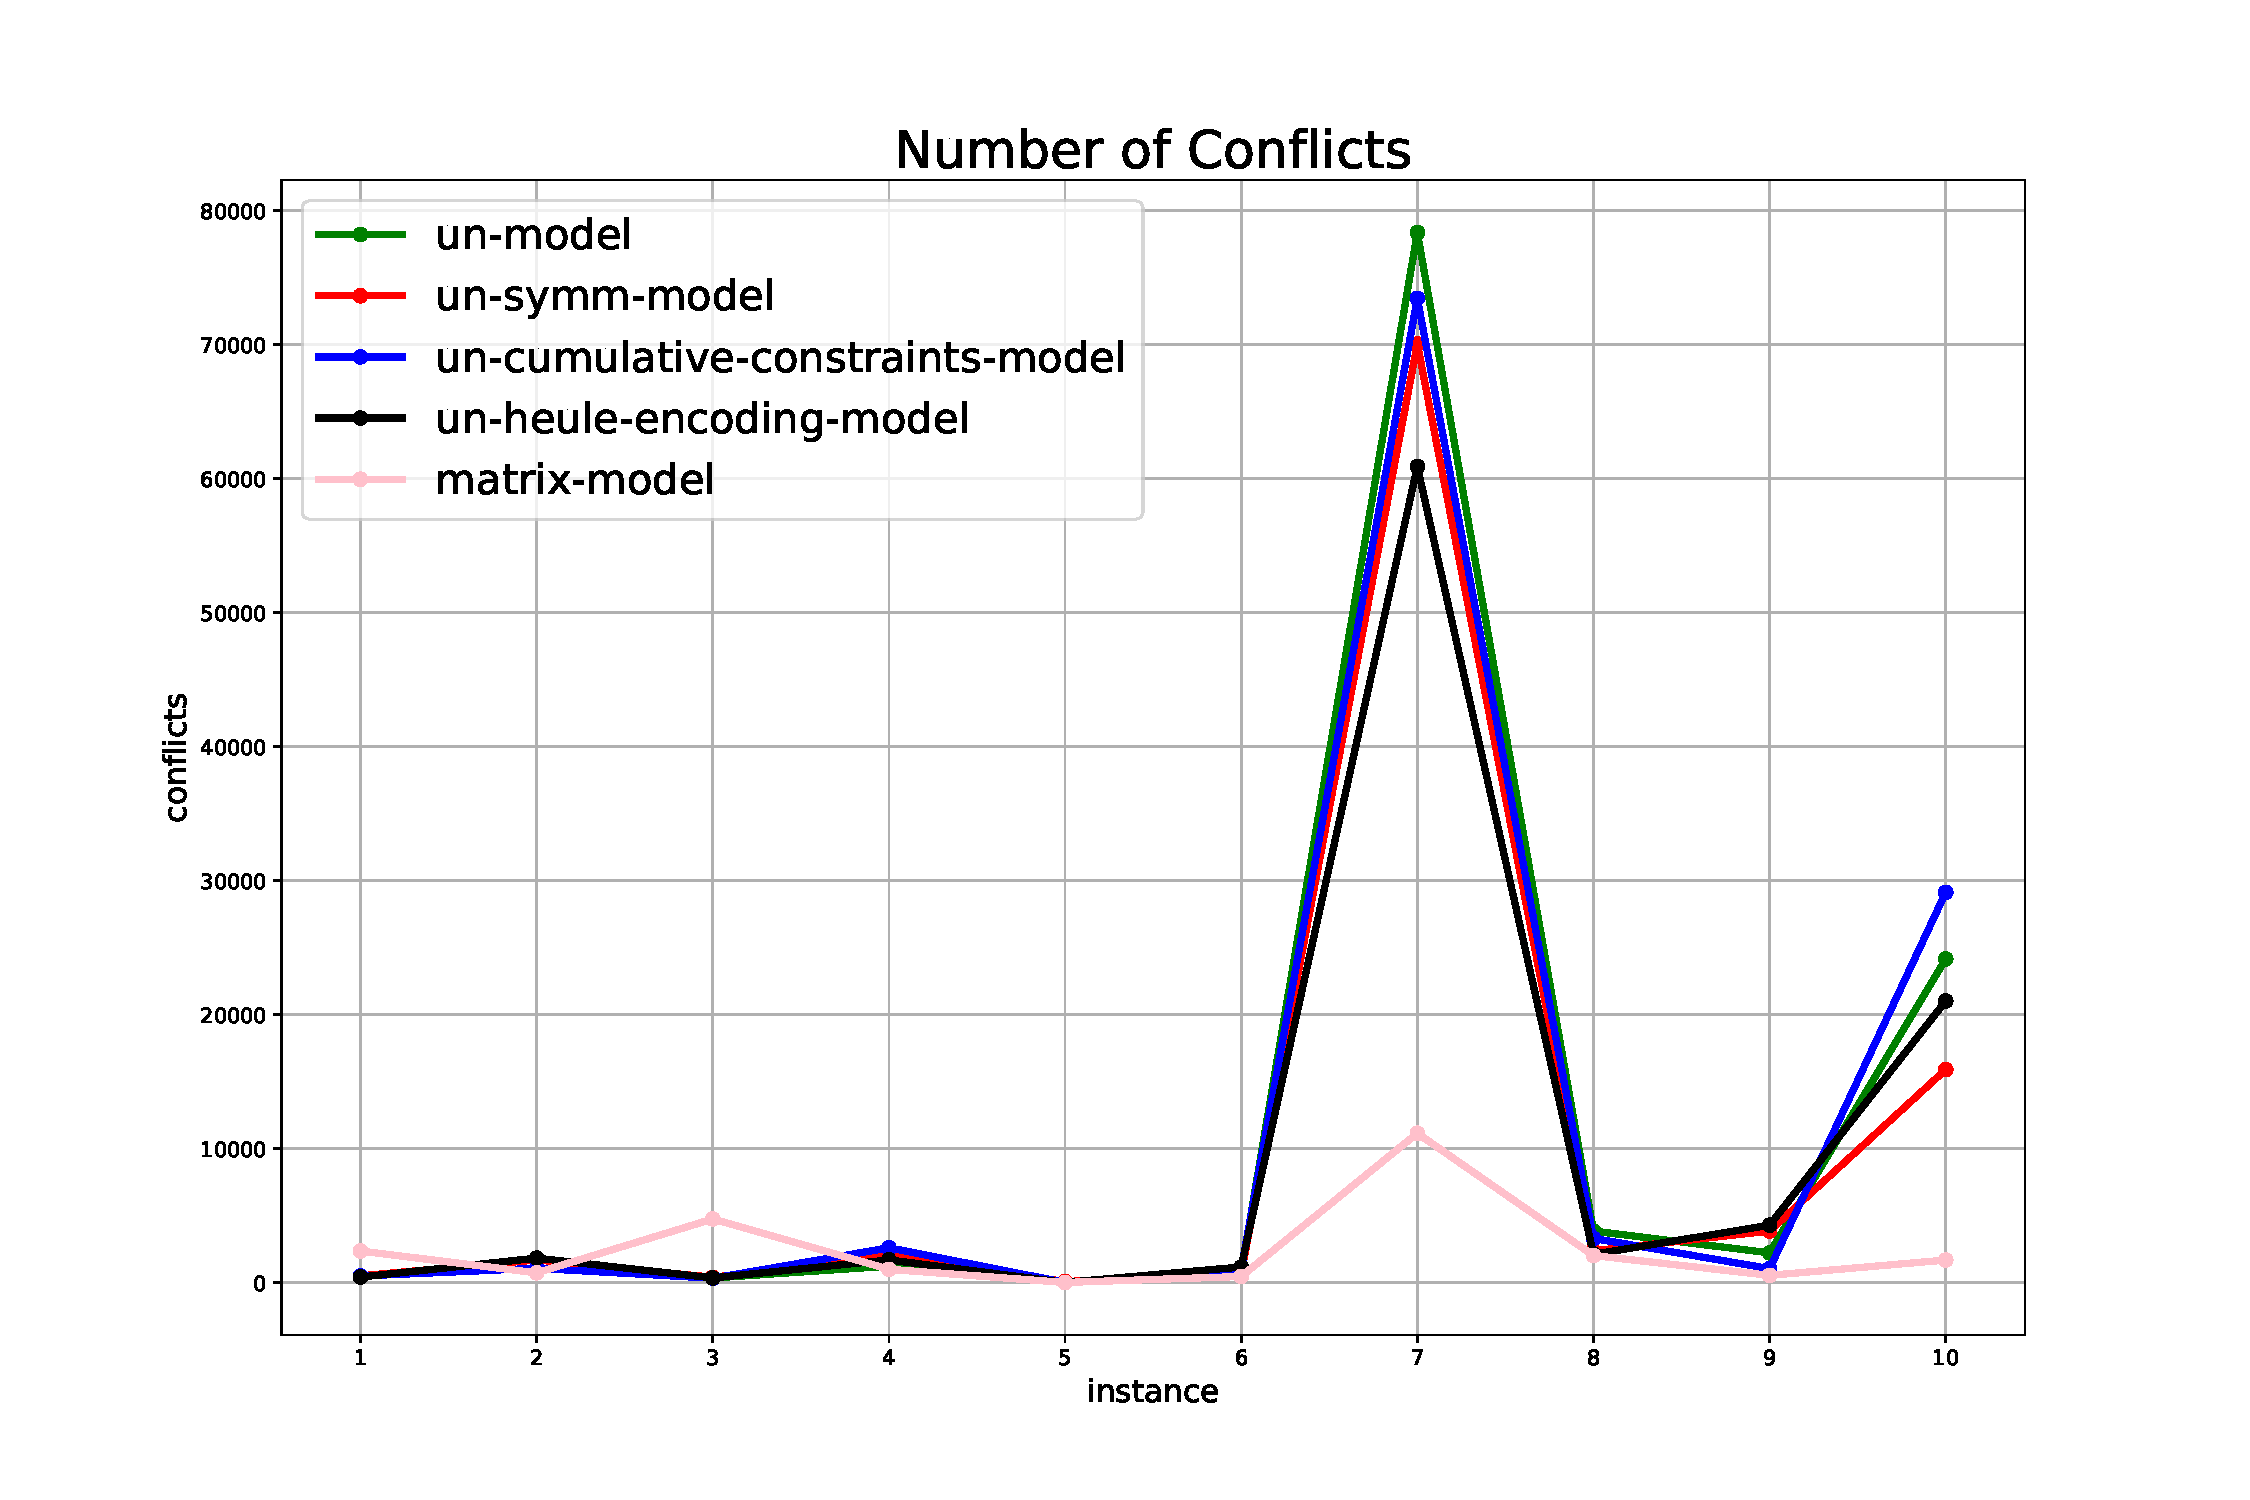
\includegraphics[width=\linewidth]{sat_images/conflicts.pdf}
        \caption{Number of conflicts for each instance}
    \end{subfigure}
    % \hfill
    % \centering
    % \begin{subfigure}{0.49\linewidth}
        % \centering
        % 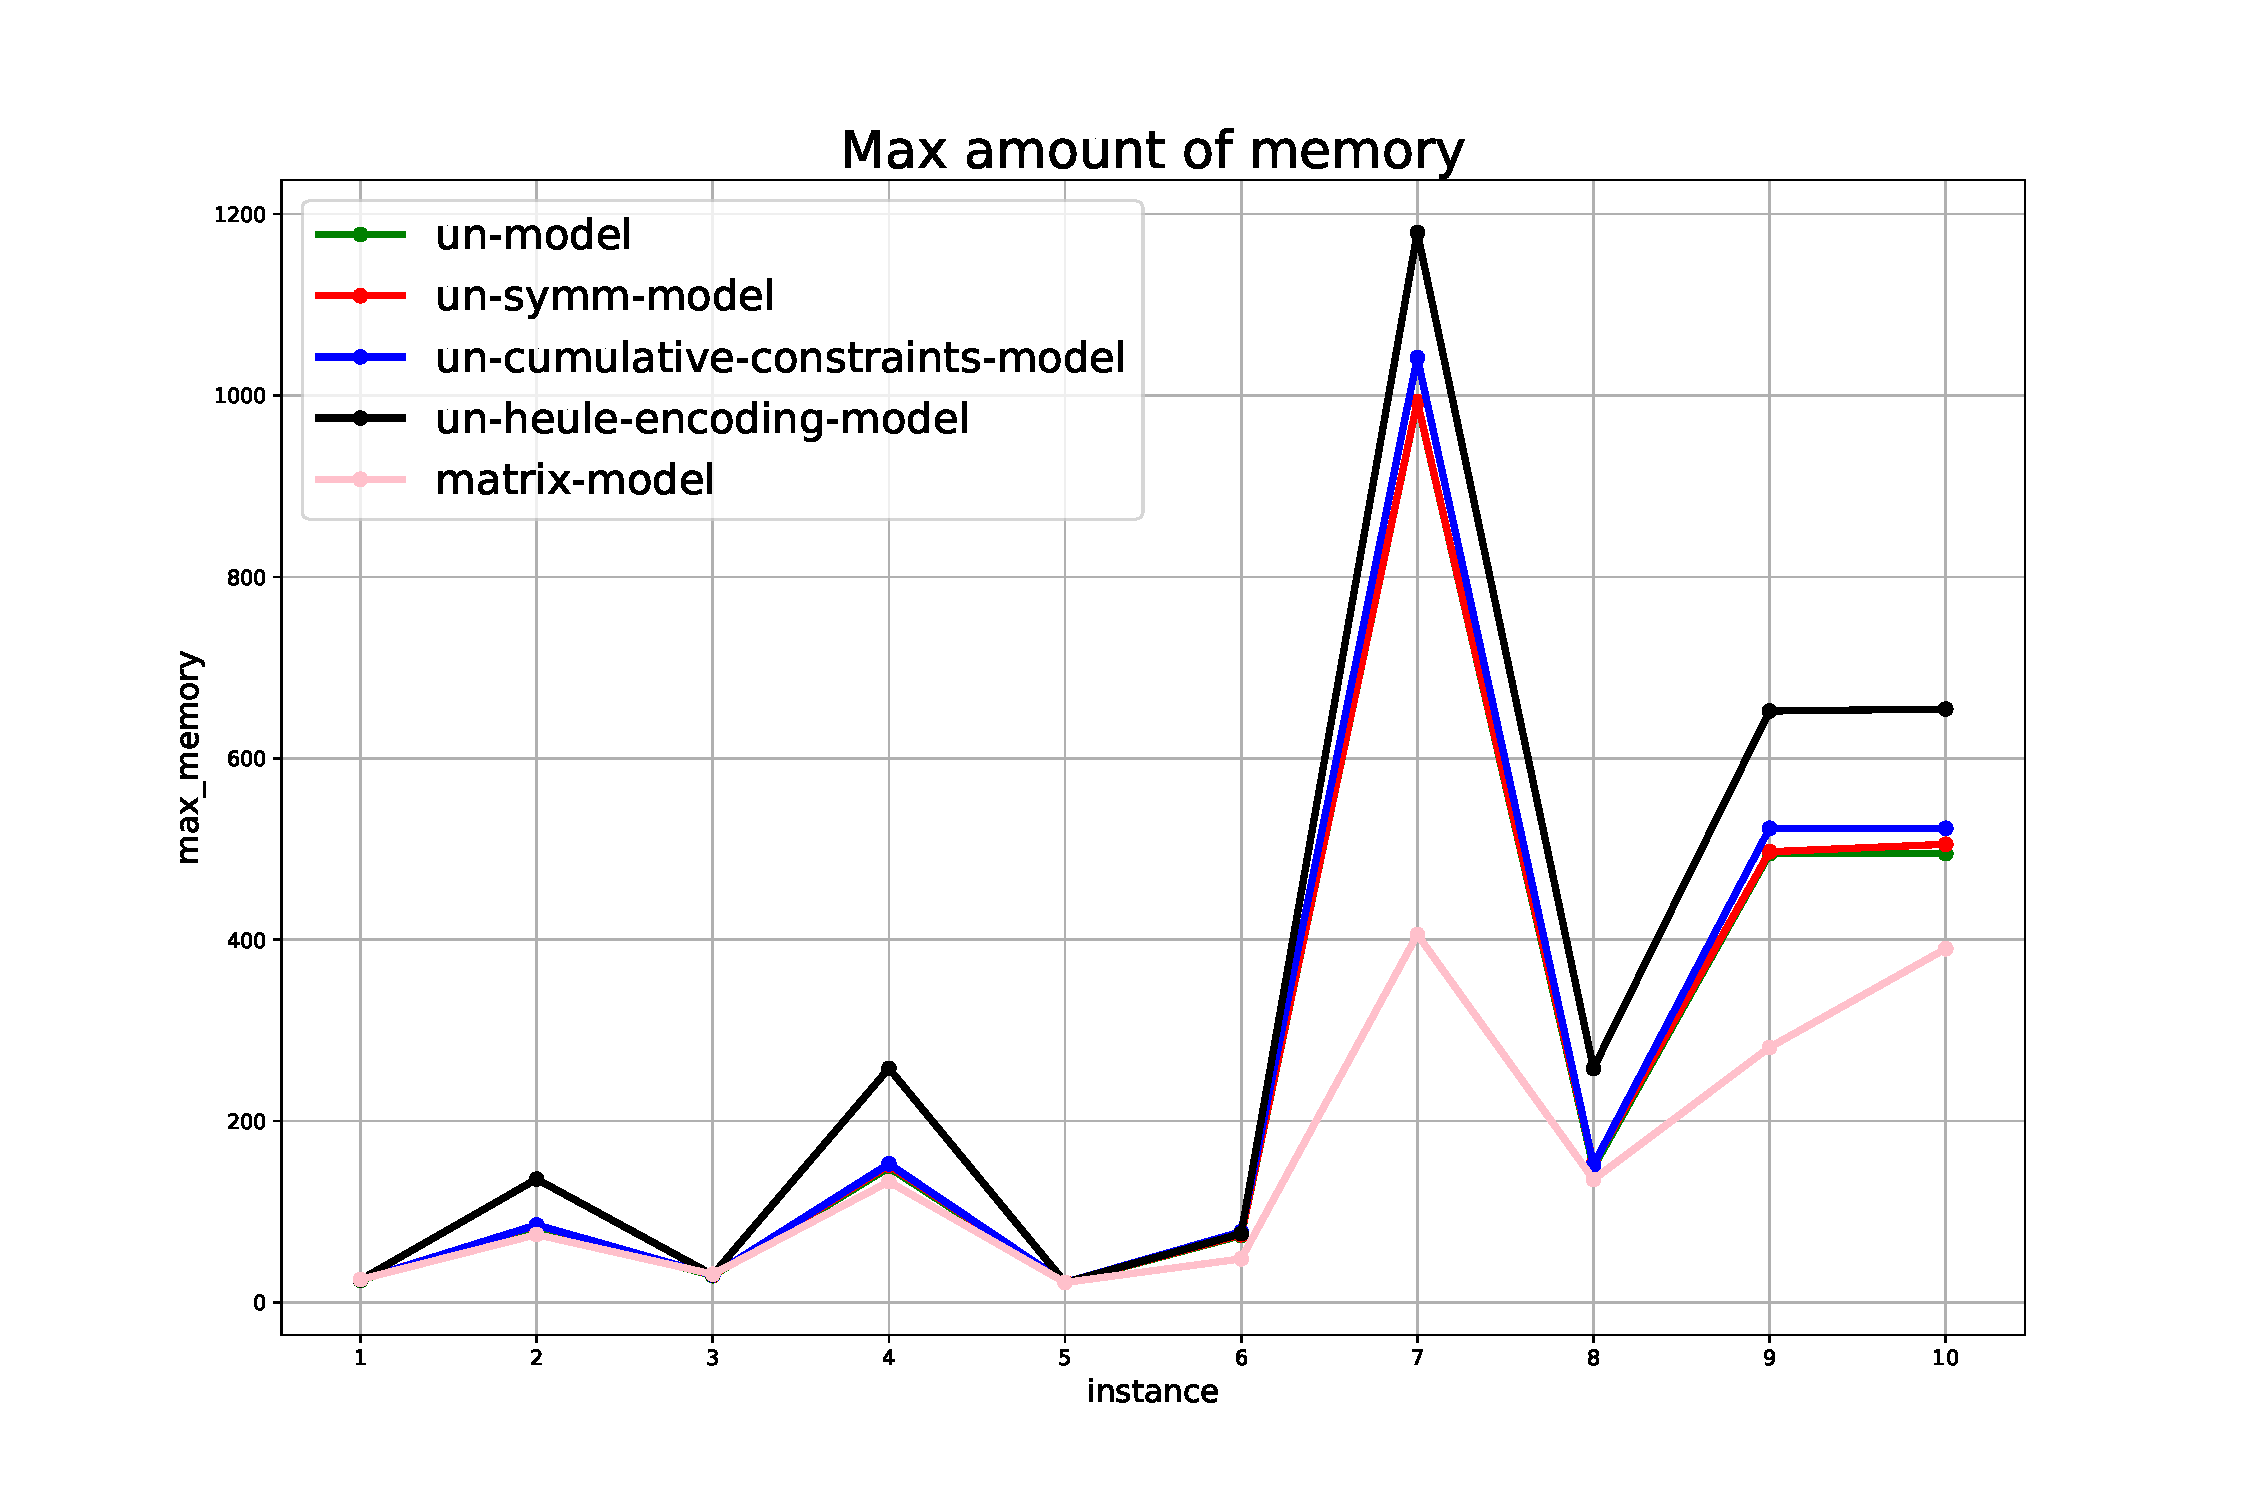
\includegraphics[width=\linewidth]{sat_images/max_memory.pdf}
        % \caption{Maximum amount of memory required for each instance}
    % \end{subfigure}
    % \hfill
    % \centering
    % \begin{subfigure}{0.49\linewidth}
        % \centering
        % 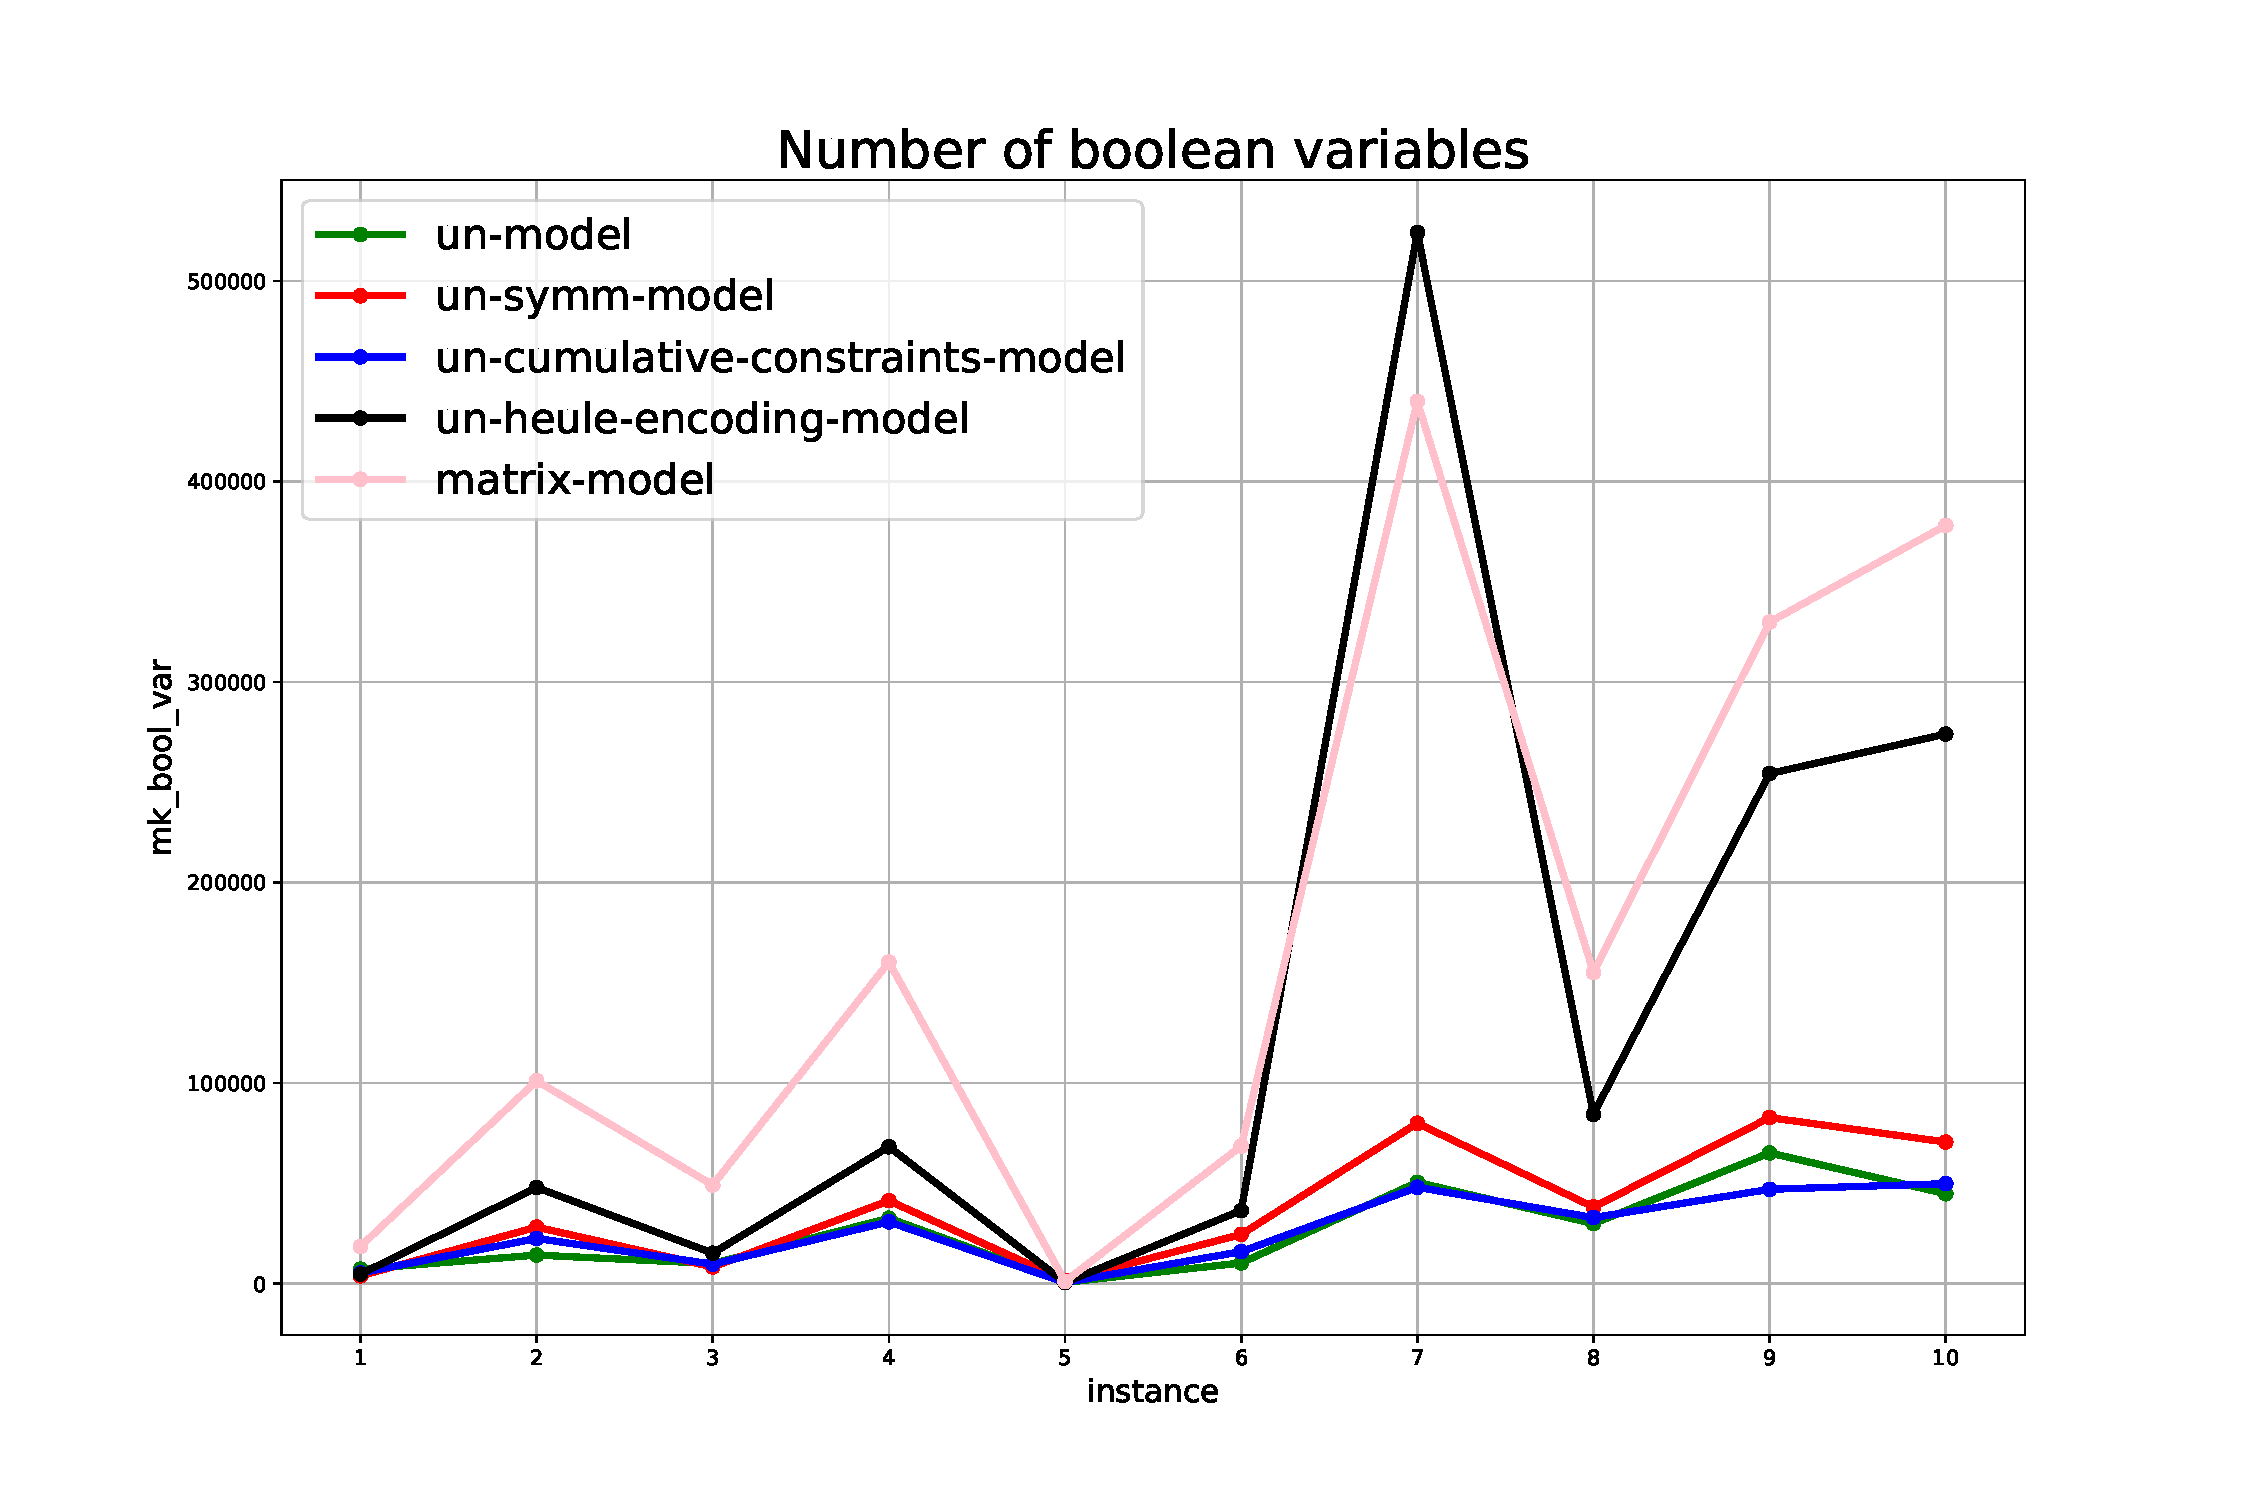
\includegraphics[width=\linewidth]{sat_images/mk_bool_var.pdf}
        % \caption{Number of boolean variables for each instance}
    % \end{subfigure}
    % \hfill
    % \centering
    % \begin{subfigure}{0.49\linewidth}
        % \centering
        % 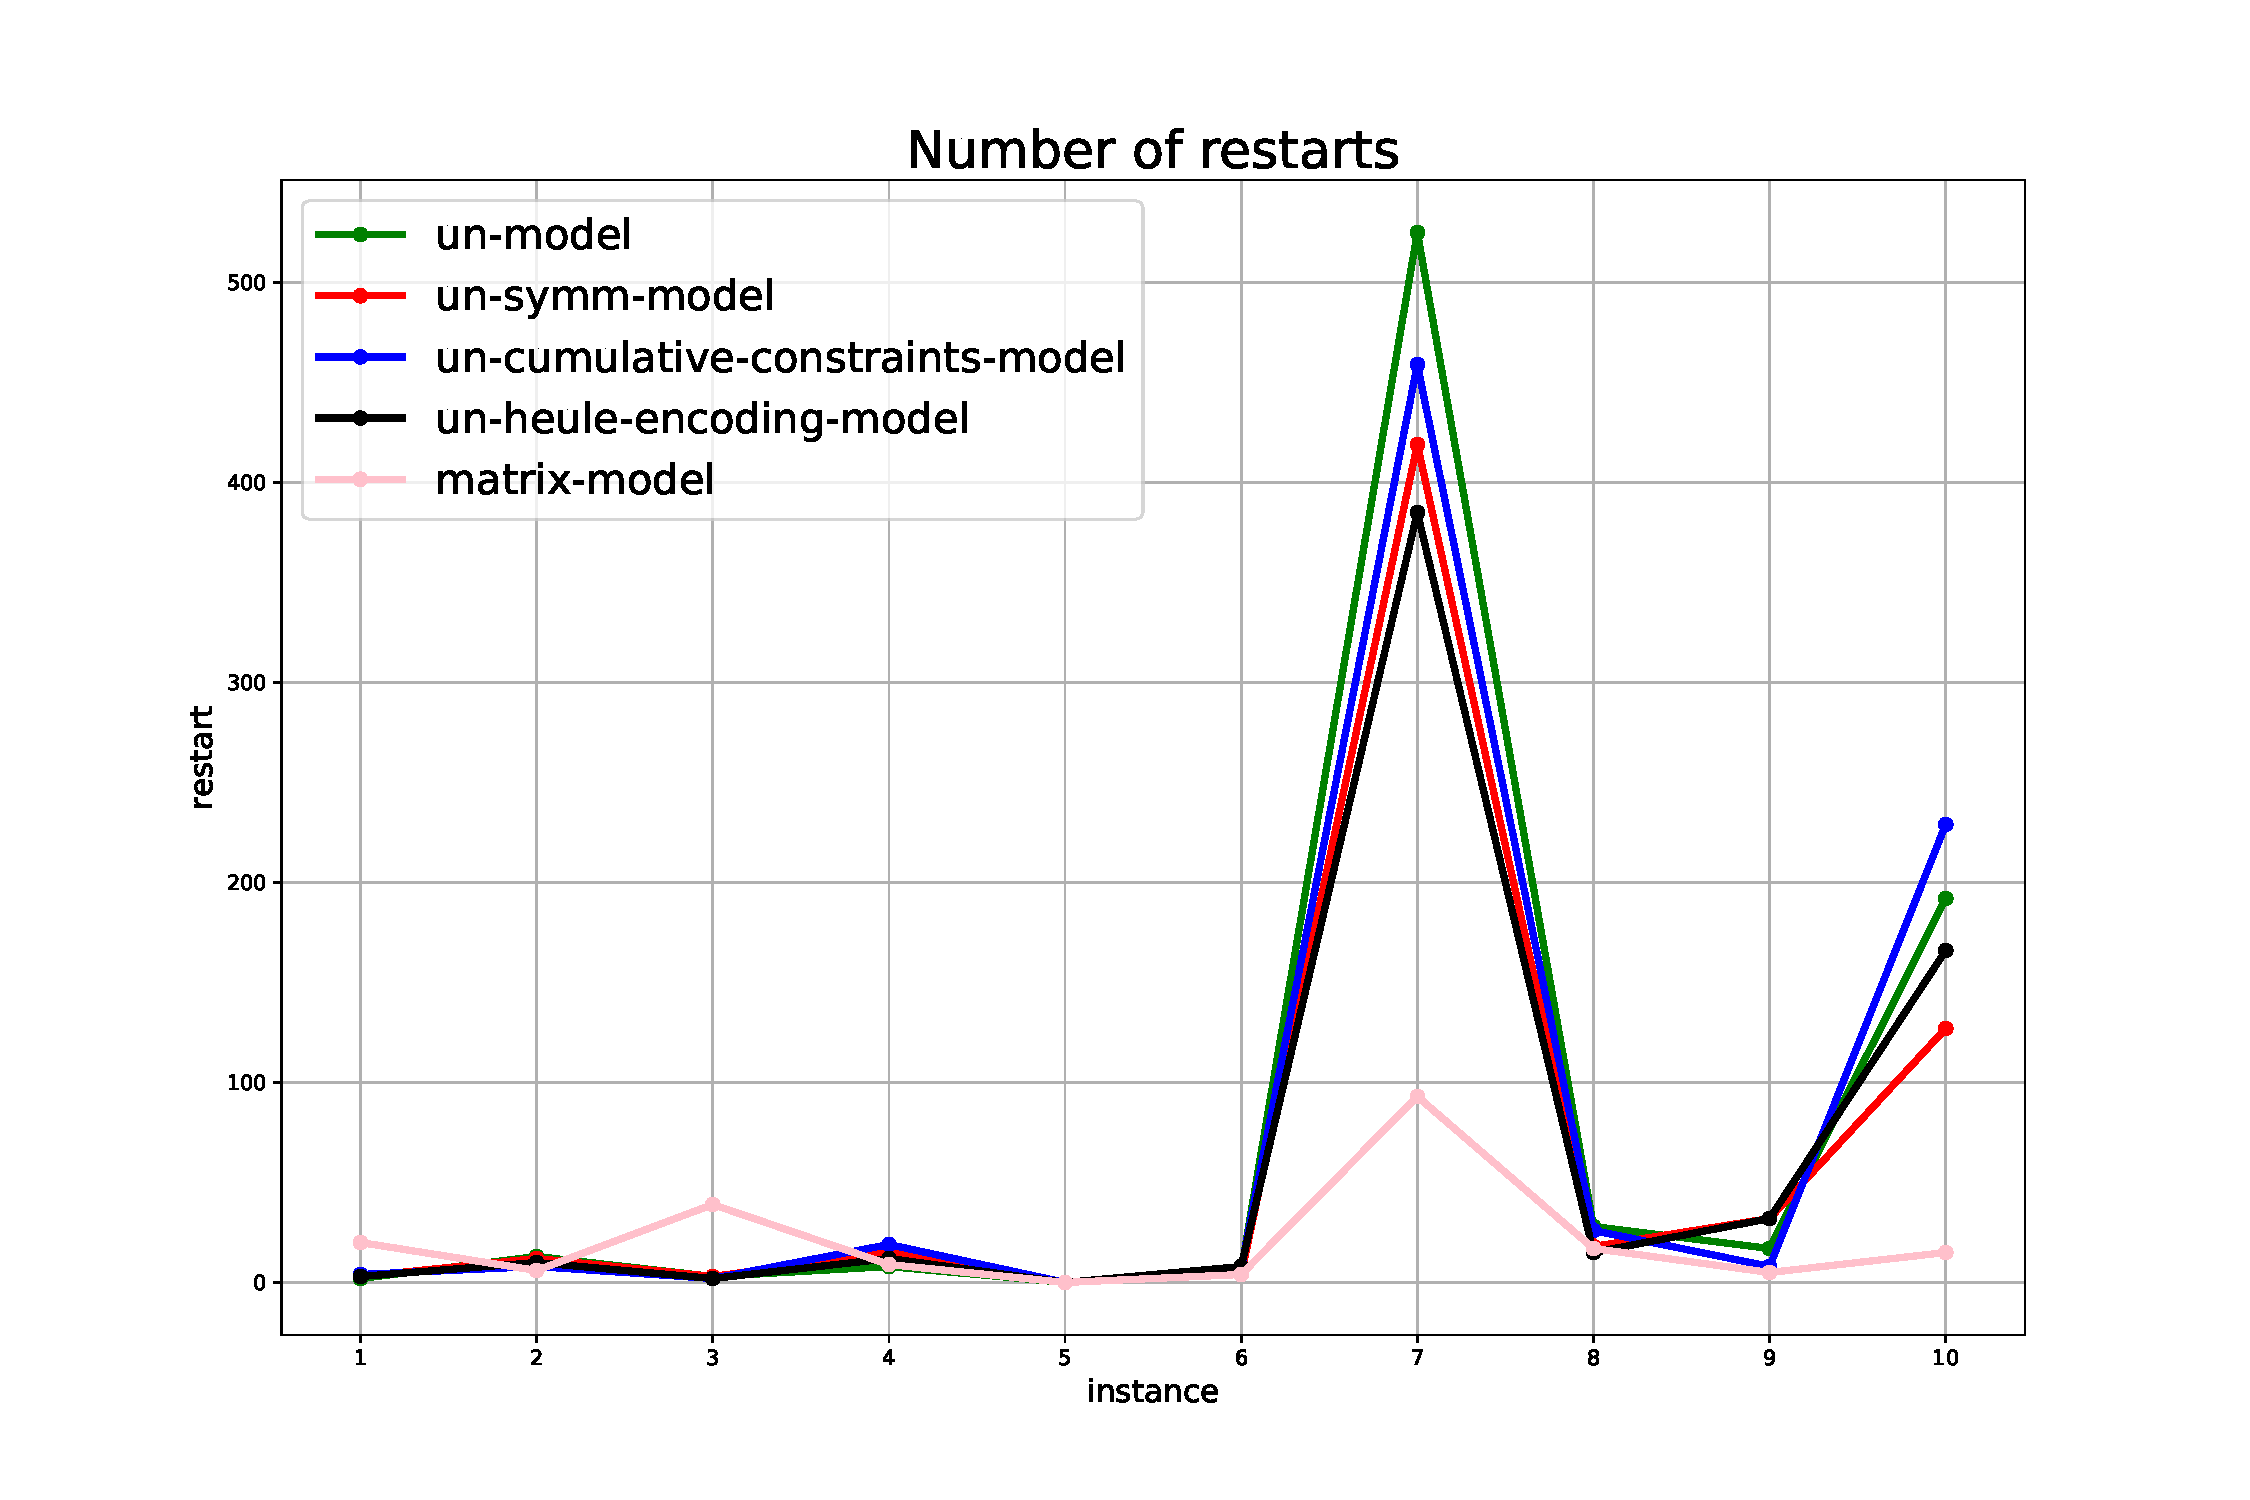
\includegraphics[width=\linewidth]{sat_images/restart.pdf}
        % \caption{Number of restarts for each instance}
    % \end{subfigure}
    \caption{Statistics about the resolution of the problem for the first 10 instances}
    \label{fig:sat_plots}\footnote{These are the only ones which reach at least a suboptimal solution.}
\end{figure}
    \section{SMT model}


\subsection{Decision variables}

The SMT model uses the logic of quantifier-free linear integer arithmetic (\texttt{QF\_LIA}) and relies on the following decision variables:

\begin{itemize}
    \item For each package $j$, $A_j \in [1, m]$ (\texttt{ASSIGNMENTS[j]} in Z3) indicates which courier delivers package $j$ where $A_j = i$ indicates that courier $i$ delivers package $j$.
    
    \item For each courier $i$, $P_{i,d} \in [1, n+1]$ for $d \in [1, n+1]$ (\texttt{PATH[i][d]} in the code) follows the definition of \Cref{eq:path_def}.

\end{itemize}

% \subsection{Auxiliary variables}
% More variables have been defined in order to make it easier to define some constraints and the objective function:

% \begin{itemize}
%     \item For each courier $i$, $D_i \in \mathbb{N}$ (\texttt{DISTANCES[i]} in Z3) is equal to the distance traveled by each courier.

%     \item For each courier $i$, $C_i \in \mathbb{N}$ (\texttt{COUNT[i]} in Z3) models the number of packages delivered by courier $i$.

%     \item For each item $j$ and for each courier $i$, $PPC_{i,j}$ (\texttt{PACKS\_PER\_COURIER[i][j]} in Z3) model the packages delivered by each courier and it is used for symmetry breaking only.
% \end{itemize}

\subsection{Objective function}
The objective function is defined as follows:

\[ \max_{i \in \{1, \dots, m\}} \texttt{DISTANCES}_i  \]
where $\texttt{DISTANCES}_i$ is equal to the distance traveled by each courier.

\subsection{Constraints}

\begin{itemize}
    \item Weight constraint: 
    \begin{equation}
        \forall i \in [1, m]: \sum_{j \in [1, n]: A_j = i} s_j \leq l_i 
    \end{equation}

    \item Assignment and path constraint:
    \begin{equation}
        \forall j \in [1, n]: \quad A_j = i \Longleftrightarrow P_{i,j} \neq j
    \end{equation}
    \begin{equation}
        \forall j \in [1, n]: \quad A_j \neq i \Longleftrightarrow P_{i,j} = j
    \end{equation}

    \item All the elements of each row of $P$ should be distinct:
    \begin{equation}
        \forall i \in [1, m]: \quad P_{i,j_1} \neq P_{i,j_2} \quad \forall j_1,j_2 \in [1, n+1], j_1 \neq j_2 
    \end{equation}

    % \item Count constraint: 

    % \begin{equation}
    %     \forall i \in \{ 1, \dots, m \}: \quad C_i = | \{ j \in \{1, \dots, n\} | A_j = i \}|
    % \end{equation}

    \item Subcircuit constraint: each row $P_i$ should define a subcircuit, that is a Hamiltonian path that ignores all the elements $P_{i,j} = j$, namely the packages that the courier $i$ don't deliver. This can be modelled through MTZ subtour elimination as defined in \Cref{eq:subtour_constr5}.

    % \item Distance constraint:
    % \begin{equation}
    %     \forall i \in \{1, \dots, m\}: \quad D_i = \sum_{j \in \{1, \dots, n+1\}} 
    %         \begin{cases}
    %             D_{j,P_{i,j}} & \text{if } P_{i,j} \neq j  \\
    %             0 & \text{if } P_{i,j} = j
    %         \end{cases}
    % \end{equation}
\end{itemize}


\subsubsection{Implied constraints}
For SMT, we experimented the implied constraint defined in \Cref{eq:impl_constr}.


\subsubsection{Symmetry breaking constraints}
For SMT, we experiment both symmetry breaking approaches as presented in \Cref{eq:cp_symm_amount,eq:cp_symm_packs}.



\subsection{Validation}


\subsubsection{Experimental design}

The experimental setup consists of two steps: first, we developed a Python package to automate the generation of SMT-LIB code from a high-level interface, allowing us to easily experiment and compare different solvers. More specifically, as solvers we experimented with Z3, cvc5, OpenSMT, SMTInterpol, and Yices 2 using both linear and binary optimization approaches. Then, to improve the performances on larger instances, we experimented with two different search strategies using the Z3 Python library (\texttt{z3py}):
\begin{description}
    \item[Two solvers approach]
        As SMT solvers do not allow to assign a priority to the variables, this approach attempts to guide the exploration of the search space by alternating two solvers: the first one finds $A$ and the second one finds $P$ given $A$. In other words, the former decides which courier delivers which package and the latter decides the route taken by each courier, basically solving $m$ different Travelling Salesman Problems. 

    \item[Local search approach]
        Similarly to the previous one, this approach also uses two solvers to first find $A$ and then $P$. However, instead of letting the second solver find an optimal solution for $P$ on its own, it is manually guided by performing a local search starting from a trivial solution (i.e., a path that delivers the items ordered by index).
\end{description}


\subsubsection{Experimental results}

The results of our experiments are presented in \Cref{tab:smt_results}. As linear optimization always outperformed binary search, we only present the former.
Analyzing SMT-LIB results, we can observe that all five solvers perform more or less similarly. The best performing is Yices 2 which solves \texttt{QF\_LIA} logic based on the simplex algorithm \cite{yices2}. On the other hand, the worst performing is SMTInterpol which relies on Craig interpolation \cite{smtinterpol}.
Furthermore, experiments in \texttt{z3py} show that symmetry breaking and implied constraints do not provide significant contribution in improving the results.

By analyzing the two search approaches, we can observe that using two separate solvers have a negligible impact on the final results with mixed effects when using symmetry breaking constraints. Instead, local search enables the model to find a solution in a reasonable amount of time, even for the largest instances.

\begin{table}[H]
    \caption{SMT results. Results in \textbf{bold} are solved to optimality. Instances that are all solved to optimality have been omitted.}
    \label{tab:smt_results}
    \centerline{
        \begin{tabular}{c|cccccccccccc}
            \toprule
            & \multicolumn{5}{c}{SMT-LIB (plain)} & \multicolumn{7}{c}{\texttt{z3py}} \\
            \\[-3ex] % Remove vertical line gap
            \cmidrule(lr){2-6} \cmidrule(lr){7-13}
            Id          & \rot{Z3}      & \rot{cvc5}    & \rot{OpenSMT} & \rot{SMTInterpol} & \rot{Yices 2} & \rot{plain}   & \rot{\makecell[l]{plain\\[-0.3em]\small+ SB}}  & \rot{\makecell[l]{plain\\[-0.3em]\small+ IC}}  & \rot{2 solvers}   & \rot{\makecell[l]{2 solvers\\[-0.3em]\small+ SB}}  & \rot{\makecell[l]{2 solvers\\[-0.3em]\small+ IC}}  & \rot{Local search}   \\ 
            \midrule                                     
            7           & 228           & 210           & 218           & 372               & \textbf{167}  & 174           & 168               & 181               & \textbf{167}      & \textbf{167}          & \textbf{167}          & \textbf{167}          \\ 
            9           & \textbf{436}  & \textbf{436}  & \textbf{436}  & 437               & \textbf{436}  & \textbf{436}  & \textbf{436}      & \textbf{436}      & \textbf{436}      & \textbf{436}          & \textbf{436}          & \textbf{436}          \\ 
            10          & \textbf{244}  & \textbf{244}  & \textbf{244}  & 381               & \textbf{244}  & \textbf{244}  & \textbf{244}      & \textbf{244}      & \textbf{244}      & \textbf{244}          & \textbf{244}          & \textbf{244}          \\ 
            11          & --            & --            & --            & --                & --            & --            & --                & --                & --                & --                    & --                    & 547                   \\ 
            12          & --            & --            & --            & --                & --            & --            & --                & --                & --                & --                    & --                    & 435                   \\ 
            13          & 1446          & --            & --            & --                & 1490          & --            & --                & --                & 1812              & 1346                  & 1832                  & 632                   \\ 
            14          & --            & --            & --            & --                & --            & --            & --                & --                & --                & --                    & --                    & 1177                  \\ 
            15          & --            & --            & --            & --                & --            & --            & --                & --                & --                & --                    & --                    & 1140                  \\ 
            16          & --            & --            & --            & --                & 1032          & --            & --                & --                & 1510              & 1944                  & 1861                  & 303                   \\ 
            17          & --            & --            & --            & --                & --            & --            & --                & --                & --                & --                    & --                    & 1525                  \\ 
            18          & --            & --            & --            & --                & --            & --            & --                & --                & --                & --                    & --                    & 917                   \\ 
            19          & --            & --            & --            & --                & --            & --            & --                & --                & --                & 870                   & --                    & 398                   \\ 
            20          & --            & --            & --            & --                & --            & --            & --                & --                & --                & --                    & --                    & 1378                  \\ 
            21          & --            & --            & --            & --                & --            & --            & --                & --                & --                & --                    & --                    & 648                   \\ 
            \bottomrule
        \end{tabular}
    }
\end{table}
    \section{MIP model}


\subsection{Decision variables}


\subsection{Objective function}


\subsection{Constraints}


\subsection{Validation}


    \section{Conclusions}

    We experimented several models using different methods and attempted to implement the same core idea across the whole project to make results comparable. Overall, all approaches are able to solve the smaller instances while, for bigger instances, only CP and SMT were able to at least produce a suboptimal solution by using proper search heuristics. Moreover, for this problem, we surprisingly observed that symmetry breaking constraints generally tend, except in a few cases, to worsen the results.

    \printbibliography

    \begin{appendices}
        \section{Implied constraint proof} \label{sec:impl_proof}
        \begin{lem}
            Assuming that the capacity of each courier allows delivering at least a package, if there exists an optimal solution, then there exists an optimal solution where each courier delivers at least one package.
        \end{lem}
        \begin{proof}
            Let us assume that the optimal solution is $D_j$ and there is a courier, say $k_1$, which do not deliver any package. Let us also suppose that the courier $k_j$ is the one that covers the maximum distance $D_j$. If we assign one package that $k_j$ brings, say $i$, to $k_1$, then, due to the triangle inequality, the two new distances $D_1$, travelled by the courier $k_1$ with $i$, and $D_2$, travelled by the courier $k_j$ without $i$, are less or equal to $D_j$. In fact:
            \begin{equation}
                \begin{split}
                    D_1 = &D[\texttt{depot},i] + D[i,\texttt{depot}] \leq\\
                        & D[\texttt{depot}, i_1] + \dots + D[i_r, i] + D[i, i_s] + \dots + D[i_t, \texttt{depot}] = D_j.
                \end{split}
            \end{equation}
            \begin{equation}
                \begin{split}
                    D_2 = &D[\texttt{depot},i_1] + \dots + D[i_r,i_s] + \dots + D[i_t, \texttt{depot}] \leq\\
                    &D[\texttt{depot}, i_1] + \dots + D[i_r, i] + D[i, i_s] + \dots + D[i_t, \texttt{depot}] = D_j.
                \end{split}
            \end{equation}
            Therefore, there are the following cases:
            \begin{itemize}
                \item If $D_1 = D_2$, either both $k_1$ and $k_j$ cover the maximum distance or neither of them do, and another courier has a route of cost $D_j$.
                \item If $D_1 > D_2$, either $k_1$ covers the maximum distance or another courier that is not $k_1$ and $k_j$ does.
                \item If $D_1 < D_2$, same as above for $k_j$.
            \end{itemize}
            So, an optimal solution still exists and has as objective value $D_j$.
        \end{proof}
    \end{appendices}

\end{document}